%TODO: Perhaps remove or add clarification
% CREATED BY DAVID FRISK, 2016

\chapter{Teori}

\section{Domänspecifika språk}
\begin{binge}
DSL $\Rightarrow$ Modellera syntax.
\end{binge}
\begin{draft}

NYA

Ett domänspecifikt språk är ett språk som är avgränsat till en specifik domän. Nyckelorden är språk, specifik och domän. Ett domän är ett område, till exempel textformatering eller matlagning. Specifikt syftar på att det är \textit{just detta} område man behandlar och inget mer. Med språk menas ett sätt att uttryck saker inom domänen. Naturliga språk kan uttrycka en uppsjö ting. Ett programmeringsspråk uttrycker instruktioner för hur en dator gör sina uppgifter.

Domänspecifika språk finns runt omkring oss i vardagen utan att vi tänker på dem. De har alltså inte nödvändigtvis med progammering att göra. Inom \textit{domänen} matlagning är steka, grilla och fritera användbara ord. Likaså inom \textit{domänen} ridning är grimma, box och galopp användbara ord. Befinner man sig inom domänen vet man vad som menas med grimma och det är ett kort och väldefinerat sätt att uttrycka sig. Men detta språk (här i form av ord/begrepp) är meningslöst utanför domänen. Ett recept kan inte förklaras i termer av grimmor, boxar och galopper.

Domänspecifika språk är vanligt förekommande i programmeringssammanhang. HTML är ett domänspecifikt språk för textformatering, SQL för databashantering och NÅT MER för NÅT MER. Samma principer som för domänspecifika språk i vardagen gäller för domänspecifika språk inom progammering. SQL är bra för databaser men inte att göra ett spel i.

Motsatsen till ett domänspecifikt språk är ett generellt språk. I vardagen är naturliga språk som svenska och engelska generella medan ryttar-begreppen ovan är domänspecifika. Likt i vardagen finns det generella programmeringsspråk som C++ och Java. Dessa är turingkompletta, vilket betyder att det kan uttrycka alla beräkningsbara problem i dem och även lösa dem givet tillräckligt med tid och \todo{referens} minnestillgångar. Begränsningen med dessa generella språk är just deras egen generaliserbarhet, eftersom de har stöd för alla typer av beräkningar så blir både läsbarheten och användarvänligheten lidande\todo{referens/motivering}.

Ett typexempel på ett domänspecifikt språk är ett \textit{syntaxträd}. Det exemplifieras här med ett syntaxträd för grundläggande matematiska uttryck, kodat i Haskell. Det visas i figur \ref{fig:syntax_exempel}.

\begin{figure}[tph]
  \begin{lstlisting}
data Expr = Expr :+: Expr
          | Expr :*: Expr
          | Const Double
  \end{lstlisting}
  \caption{Ett syntaxträd i Haskell. Detta är ett exempel på ett litet domänspecifikt språk.}
  \label{fig:syntax_exempel}
\end{figure}

Ett syntaxträd innehåller \textit{datakonstruktorer} för att representera \textit{löv} (ändpunkter) och \textit{förgreningar}. I detta exempel är \texttt{:+:} och \texttt{:*:} förgreningar. Med hjälp av dem kan man uttrycka summan respektive produkten av två \textit{andra} uttryck. \texttt{Const} är ett löv. Det är här en konstant som man ej kan bygga vidare på.

Med datakonstruktorerna kan man konstruera värden i språket. Ett exempelvärde från det tidigare syntaxträdet visas i figur \ref{fig:syntax_exempel_varde}.

\begin{figure}[tph]
  \begin{lstlisting}
value = Const 7 :*: (Const 3 :+: Const 10)
  \end{lstlisting}
  \caption{Ett exempelvärde ur det tidigare syntaxträdet. Detta modellerar det matematiska uttrycket $7 * (3 + 10)$}
  \label{fig:syntax_exempel_varde}
\end{figure}

Figur \ref{fig:syntax_exempel_varde} visar hur det matematiska uttrycket $7 * (3 + 10)$ modelleras. Konstruktorn \texttt{:*:} får som sina två argument uttrycken \texttt{Const 7} och \texttt{Const 3 :+: Const 10}. Det är alltså en produkt av två deluttryck. Syntaxträd brukar illusteras med just träddiagram. Detta exempelvärde illustreras i figur \ref{fig:syntax_exempel_bild}.

\begin{figure}[tph]
  \centering
  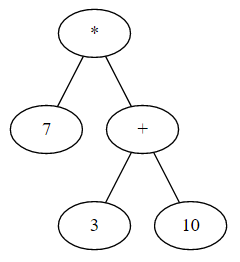
\includegraphics[width=0.4\linewidth]{figure/syntax_exempel_bild.png}
  \caption{Exempelvärde från syntaxträdet illustrerat i ett träddiagram.}
  \label{fig:syntax_exempel_bild}
\end{figure}

Ett domänspecifikt språk kan antingen implementeras som ett fristående språk eller bäddas in i ett redan existerande språk. De domänspecifika språk som   utvecklats inom detta projekt är inbäddade i språket Haskell.

GAMLA


  Ett domänspecifikt programmeringsspråk är ett språk som är avgränsat till ett
  specifikt domän. Detta domän kan ta många former, det kan vara ett språk för
  att formatera text på en hemsida (HTML), det kan vara ett språk för att
  interagera med en databas (SQL), ett språk för ett beskriva hur text ska se
  ut på en skärm  (typsnitt). Användningsområden för dessa språk är väldigt
  smala men detta smala fokus gör det möjligt att utveckla ett rikt och
  lättanvändligt språk för just detta område.

  Motsatsen till ett domänspecifikt språk är ett generellt språk (C, Java,
  Python) vilka är turingkompletta, vilket betyder att det kan uttrycka alla
  beräkningsbara problem i dem och även lösa dem givet tillräckligt med tid och
  \todo{referens} minnestillgångar. Begränsningen med dessa generella språk är
  just deras egen generaliserbarhet, eftersom de har stöd för alla typer av
  beräkningar så blir både läsbarheten och användarvänligheten lidande\todo{referens/motivering}.

  Ett domänspecifikt språk kan antingen implementeras som ett fristående språk
  eller bäddas in i ett redan existerande språk. De domänspecifika språk som
  utvecklats inom detta projekt är inbäddade i språket \textit{Haskell}.
\end{draft}

\section{Det funktionella programmeringsspråket Haskell}

\begin{binge}
  Haskell är ett funktionellt programmeringsspråk som lämpar sig bra för att
  implementera ett domänspecifikt språk i. Anledningen till detta är den lätthet
  som man kan skapa nya datatyper och klasser för att representera grundstenarna
  i det nya språk, och även dess mönstermatchning som gör det möjligt att på
  enkelt sätt bryta isär komplexa datatyper för evaluering.

  TODO: Visa exempel på detta
\end{binge}

\section{Syntaxträd och deras evaluering}

Ska kanske slås ihop med DSL-avsnittet, då syntaxträd är ett så bra exempel på DSL

Ett typexempel på ett domänspecifkt språk är ett syntaxträd för algebraisk uttryck, här kodat i Haskell.



I detta exempel visar hur uttrycket $(7+x)*((x+10)*x)$ kodas.

Ha med en bild på detta.

!!!Plus förklaring om evaluering!




\section{Litterat programmering och Literate Haskell}
\label{sec:lhs}
\begin{draft}
\textit{Litterat programmering} (engelska \textit{literate programming}) är ett
alternativt sätt att programmera som introducerats av Donald Knuth.\cite{knuth}
Istället för att skriva ett program för en dator, skriver man ett program som
ska läsas av människor. Det visar sig på följande två sätt.

Det en sättet är att jämfört med traditionella program får dokumentationen en
ökad betydelse. I traditionella program är programkoden den viktiga delen. I
litterata program däremot är dokumentationen minst lika viktig. Den anänds till
att förklara koden, sätta den i relationen till andra delar och så vidare.
Detta jämnbördiga förhållande syns konkret genom att titta på hur källkoden är
skriven i ett literat program. Det kan till exempel se ut som i figur
\ref{fig:litterate_haskell_exempel} där man ser att källkod och text för
människor är sammanvävda på ett jämnbördigt sätt, där den ena inte är viktigare
än den andra.

\begin{figure}[tph]
  \begin{lstlisting}[language={}]
How does all this tie together? First the type is decided, for instance

< type ExampleType = Quantity T.Length Double

then a value of that type is created

< exampleValue :: ExampleType
< exampleValue = Quantity V.length 5.3

Note that the Quantity data type has both value-level and type-level dimensions. As previosuly mentioned, value-level in order to print prettily and type-level to only permit legal operations.
  \end{lstlisting}
  \caption{Ett exempel på hur en källfil till litterat programmering kan se ut. Exemplet är Litterate Haskell. Rader som börjar med \texttt{<} markerar att det är progamkod, medan rader utan markerar att det är text för människor.}
  \label{fig:litterate_haskell_exempel}
\end{figure}
%TODO: programraderna brukar väl börja med ">" inte "<"?

Det andra sättet ett litterat program skiljer sig åt är ordningen progamkod
står i. Traditionellt används top-down eller bottom-up. Dessa tillvägagånssätt
står i kontrast till den som används i litterat programmering, där man
betraktar ett program som ett nät av många delar som hänger ihop, utan att de
nödvändigvis har en övergripande hierariki som de tradionella metoderna bygger
på. Detta uttnyttjas genom att då presentera progamkoden i den ordning som är
lättast att förstå för den mänskliga läsaren.

\textit{Litterate Haskell} är literat programmering för Haskell.\cite{litterate_haskell}
Att progammera i Litterate Haskell går till på samma sätt som vanlig Haskell,
med skillndaden att programkod och text vävs ihop i en och samma fil. Det kan
se ut som i figur \ref{fig:litterate_haskell_exempel}. Filen, med tillägget
\texttt{.lhs}, går att använda direkt med Haskell-kompilatorn GHC. All text
ignoreras och programkoden behandlas som om den tillhörde en vanlig
Haskell-fil. \texttt{.lhs}-filen kan också kompileras till material avsett för
mäniskor. Det finns flera verktyg som gör det men det som används i detta
projekt är \textit{Pandoc}\cite{pandoc}. Med \textit{Pandoc} kan texten märkas
up med både \texttt{markdown} (används i projektet) och \texttt{Latex}. Det går
att exportera till bland annat HTML och PDF.  \end{draft}

\section{ARCS/didaktik}
\label{sec:arcs}
% TODO: använd inte förkortningen i rubriken.


\begin{binge}

Lärande Skola Bildning - kap 5 lärandeteorier

Knyta an materialets undervisningspotential till lärandeteorier.

Vygotskij - Sociokulturella lärandet (ex parprogrammering + diskussion emellan individer)

Jean Piaget - Kognitivismen (lära sig A, B, A + B -> C, alternativt att eleven utmanas med något den trodde var sant, och tvingas omformulera en lösning som stödjer den presenterade situationen).

Skinner - Behaviorism (ex glada tomater vs wall of text? Det är väll egentligen detta som hindrar läsare att läsa en "tråkig, tung svårläst text")
Vi väver in det som elever inte förknippar med tunga texter -> färre flyktförsök.

\iffalse
Skulle vilja hitta stöd för:
Bara något som olika bakgrunder skulle kunna ge en inbillning av miljöombyte, vilket minskar den monotona dimensionen, och i sig förhindrar hjärnans anti-"get-stuck-on-a-thought-and-die".
\fi

\end{binge}
